\section{Periodic Repetition (TODO RENAME THIS?}
\subsection{Improvement Goals}
A description for periodic boundary conditions is given in \cref{pbc_explain} regarding how a small simulation box simulates a subset of an infinite lattice. It may be useful to visualise a larger subset of this infinite lattice by repeating the simulation box a number of times. Additionally, the capability of repeating a smaller system is useful for producing a realistic, much larger configuration for testing the performance of WebMGA with increased molecule counts due to the lack of availability of real test configurations of such sizes.

\subsection{WebMGA 3.0 Implementation}
A few modifications needed to be made to implement this feature.

First, the ``reference'' tab in the side menu was modified to include inputs for the repeat count in the `x' `y' and `z' directions. With a value of zero, there should be only a single instance of the configuration along the corresponding axis. Setting to one adds a repeat in the positive and negative direction along the axis, with bounding box faces touching (i.e. with a value of 0, there will be 1 instance of the configuration, with 1 there will be 3 instances, 2 there will be 5 instances etc.). When multiple directions have a value larger than 0, the configurations are repeated such that a single large box is produced (i.e. it is ensured there are no gaps, for example a configuration of $(1,1,1)$ will give a box of dimensions $3\times 3\times 3$ with $27$ total instances of the initial configuration).

Repetition of the configuration was implemented by changing TODO FINISH THIS

\begin{figure}
  \begin{center}
    \begin{subfigure}{0.3\textwidth}
      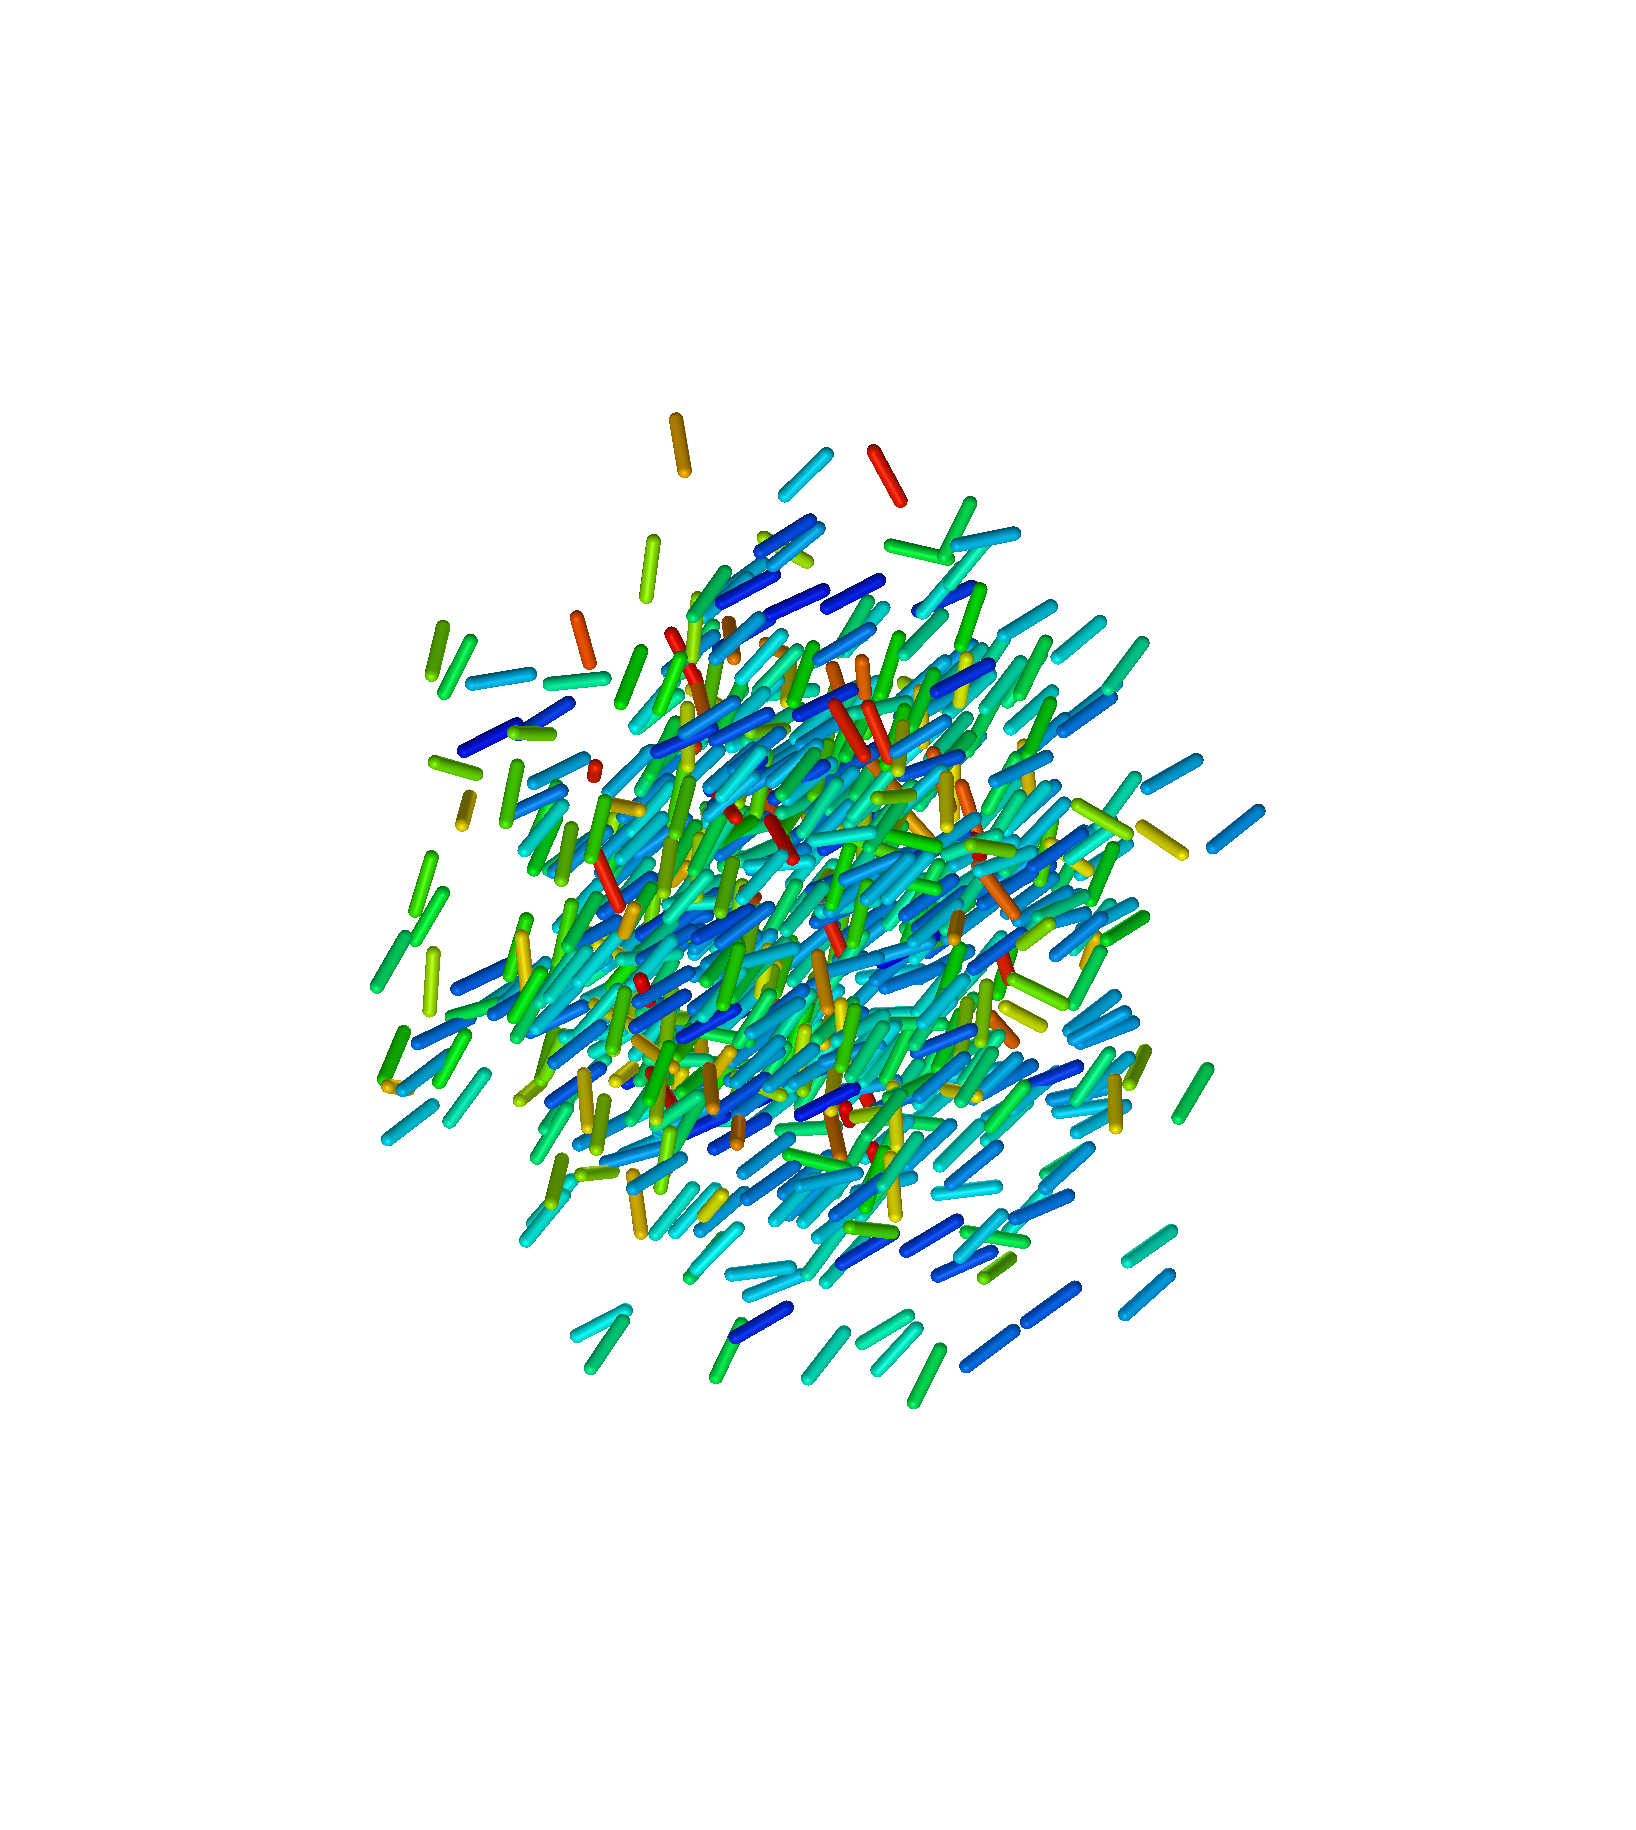
\includegraphics[width=\textwidth]{assets/images/periodic/1}
      \caption{$(0,0,0)$}
      \label{fig:periodic_1}
    \end{subfigure}
        \begin{subfigure}{0.3\textwidth}
      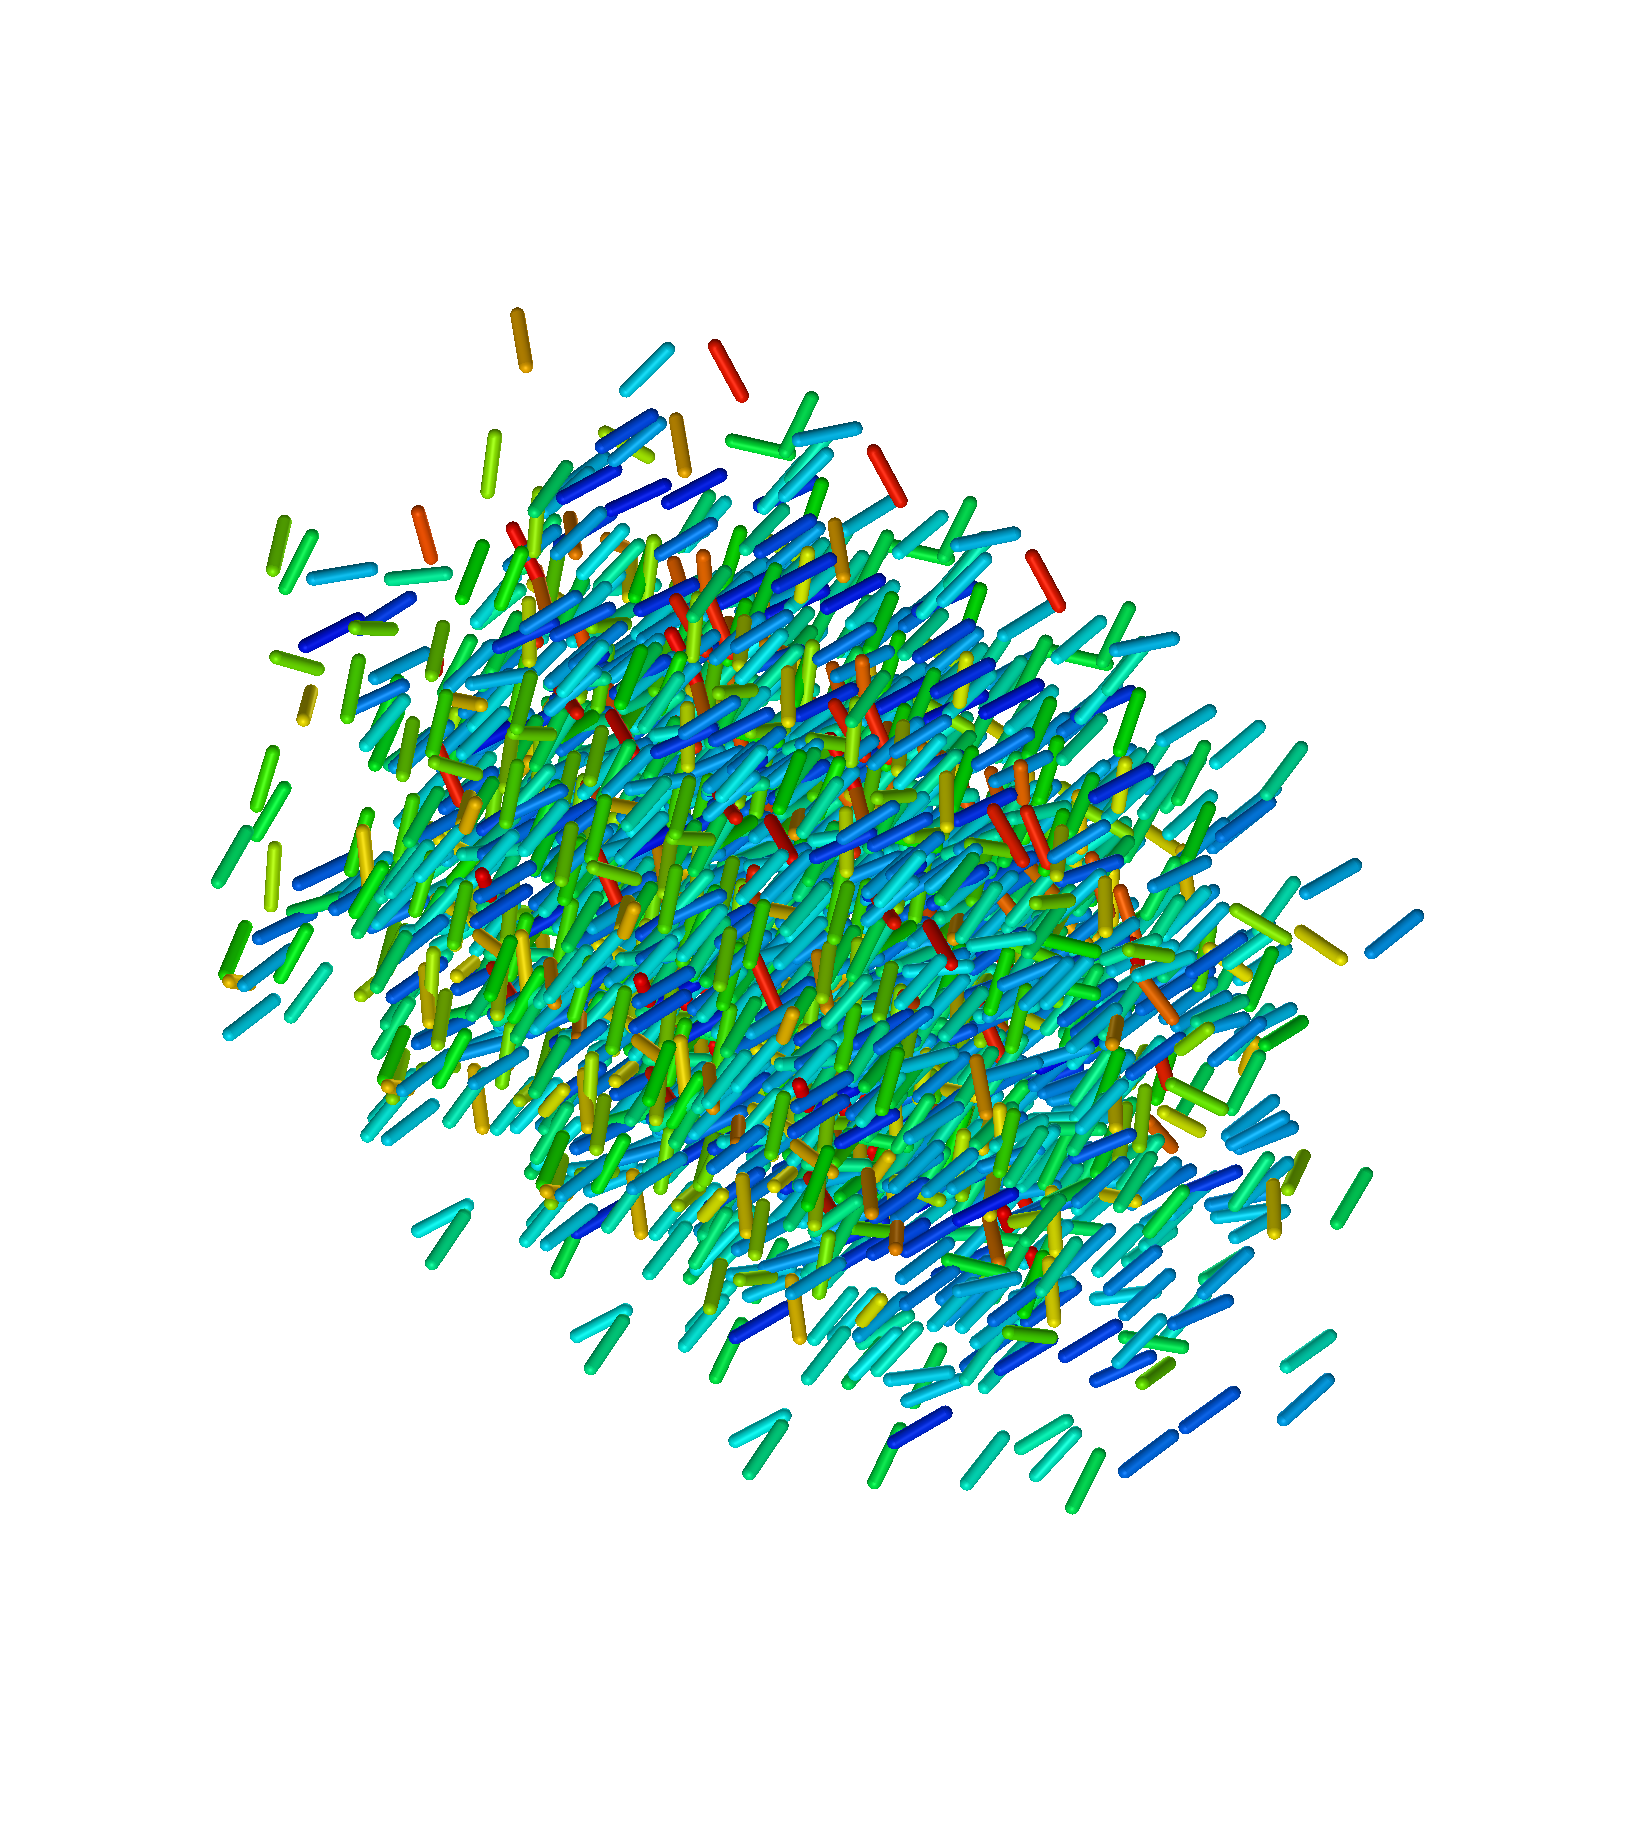
\includegraphics[width=\textwidth]{assets/images/periodic/2}
      \caption{$(1,0,0)$}
      \label{fig:periodic_2}
    \end{subfigure}
        \begin{subfigure}{0.3\textwidth}
      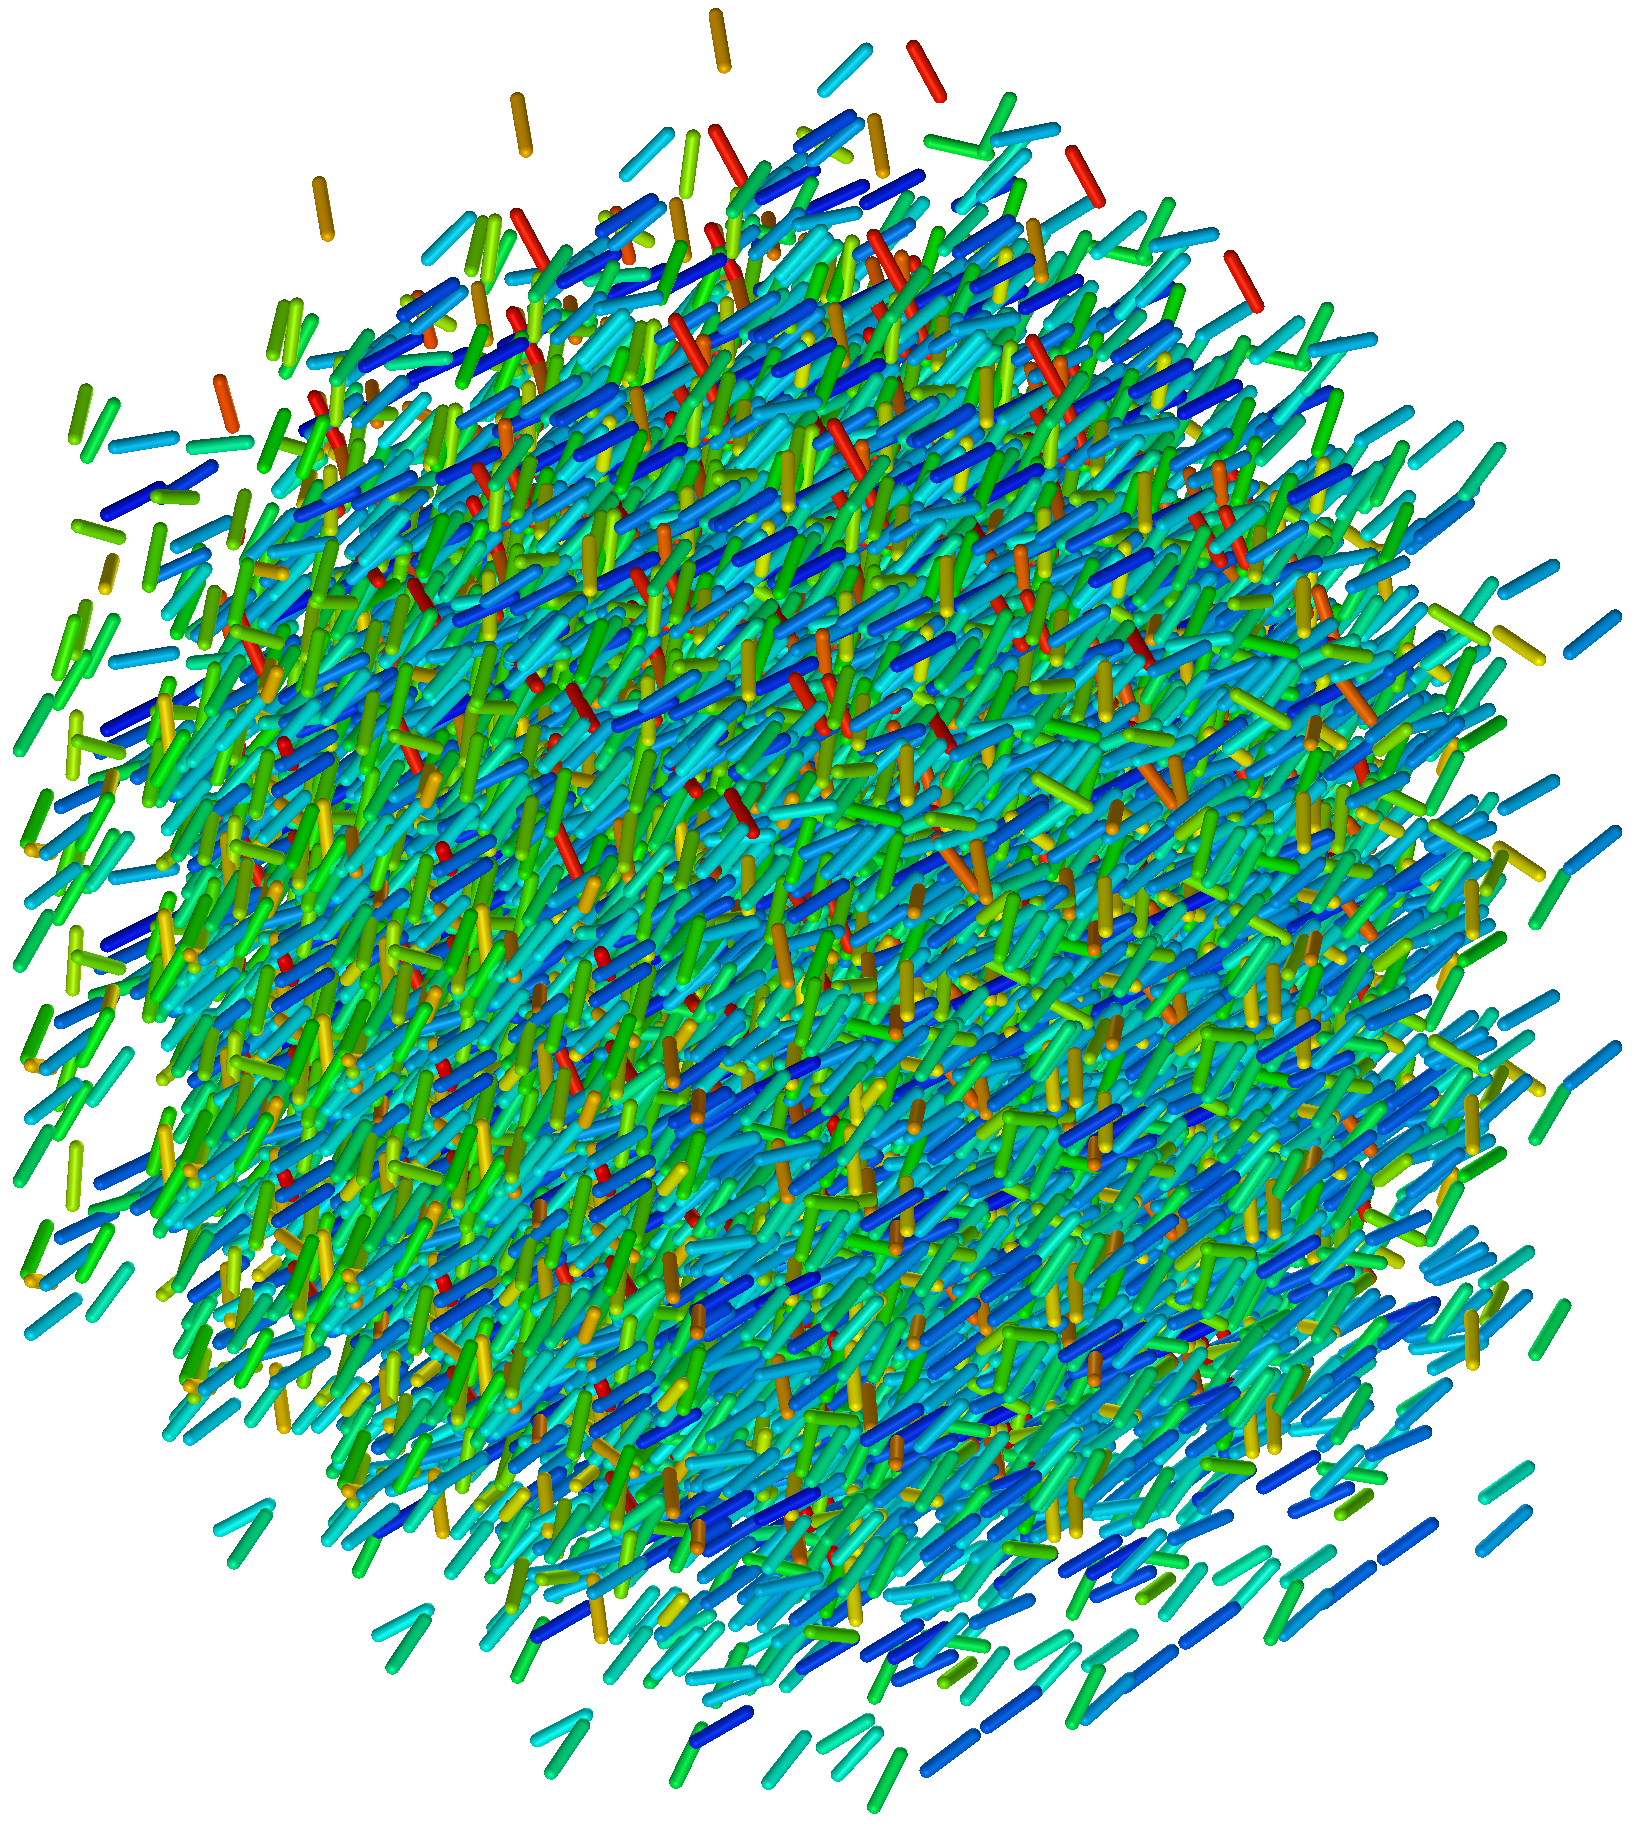
\includegraphics[width=\textwidth]{assets/images/periodic/3}
      \caption{$(1,1,1)$}
      \label{fig:periodic_3}
    \end{subfigure}
  \end{center}
  \caption{Demonstration of periodic repetition of a configuration, labelled with repetition parameter of format $(x, y, z)$.}
  \label{fig:periodic}
\end{figure}

\subsection{WebMGA 3.0 Bugs}
TODO
